\section{Experiments}
\label{sec:experiments}

The empirical evaluation of \texttt{Active-Bidder} aims to demonstrate that treating real-time bidding (RTB) as an active inference process provides superior long-term utility compared to traditional discriminative or reward-based reinforcement learning (RL) frameworks. Our experimental design is structured as a quest to prove three primary hypotheses: (i) the minimization of Variational Free Energy (VFE) corresponds to the emergence of a robust internal world model of user behavior; (ii) the principled integration of epistemic value allows the agent to sacrifice immediate click-through rates (CTR) for superior long-term value (LTV); and (iii) the method maintains stability under the high-volatility conditions characteristic of digital advertising auctions.

\subsection{Experimental Setup and Baselines}

We evaluate our framework using a high-fidelity RTB simulator built upon the \textit{Criteo Ad-logs} and \textit{Avazu} datasets \cite{diemert2018criteo}, augmented with a temporal decay function to simulate long-term user retention and LTV. The environment consists of a continuous stream of bid requests where the state $\mathbf{s}_t \in \mathcal{S}$ includes user historical features, contextual metadata, and remaining budget. The action $\mathbf{a}_t \in \mathbb{R}^+$ represents the bid price.

We compare \texttt{Active-Bidder} against three classes of baselines:
\begin{enumerate}
    \item \textbf{Heuristic/Linear}: LinUCB \cite{li2010contextual}, a standard contextual bandit approach that balances exploration via upper confidence bounds but lacks a temporal horizon.
    \item \textbf{Reinforcement Learning}: PPO (Proximal Policy Optimization) \cite{schulman2017proximal}, representing the state-of-the-art in model-free RL for bidding, which optimizes for a discounted reward sum.
    \item \textbf{Generative Baselines}: A Variational Autoencoder (VAE) based bidding strategy that models user distributions but lacks the active inference control loop.
\end{enumerate}

\subsection{Convergence Analysis of Variational Free Energy}

The fundamental objective of \texttt{Active-Bidder} is the minimization of the Variational Free Energy $\mathcal{F}$, which serves as an upper bound on the ``surprise'' or negative log-evidence of the observed auction outcomes. Figure \ref{fig:vfe_convergence} illustrates the convergence trajectory of $\mathcal{F}$ over $10^6$ training iterations.

\begin{figure}[htbp]
    \centering
    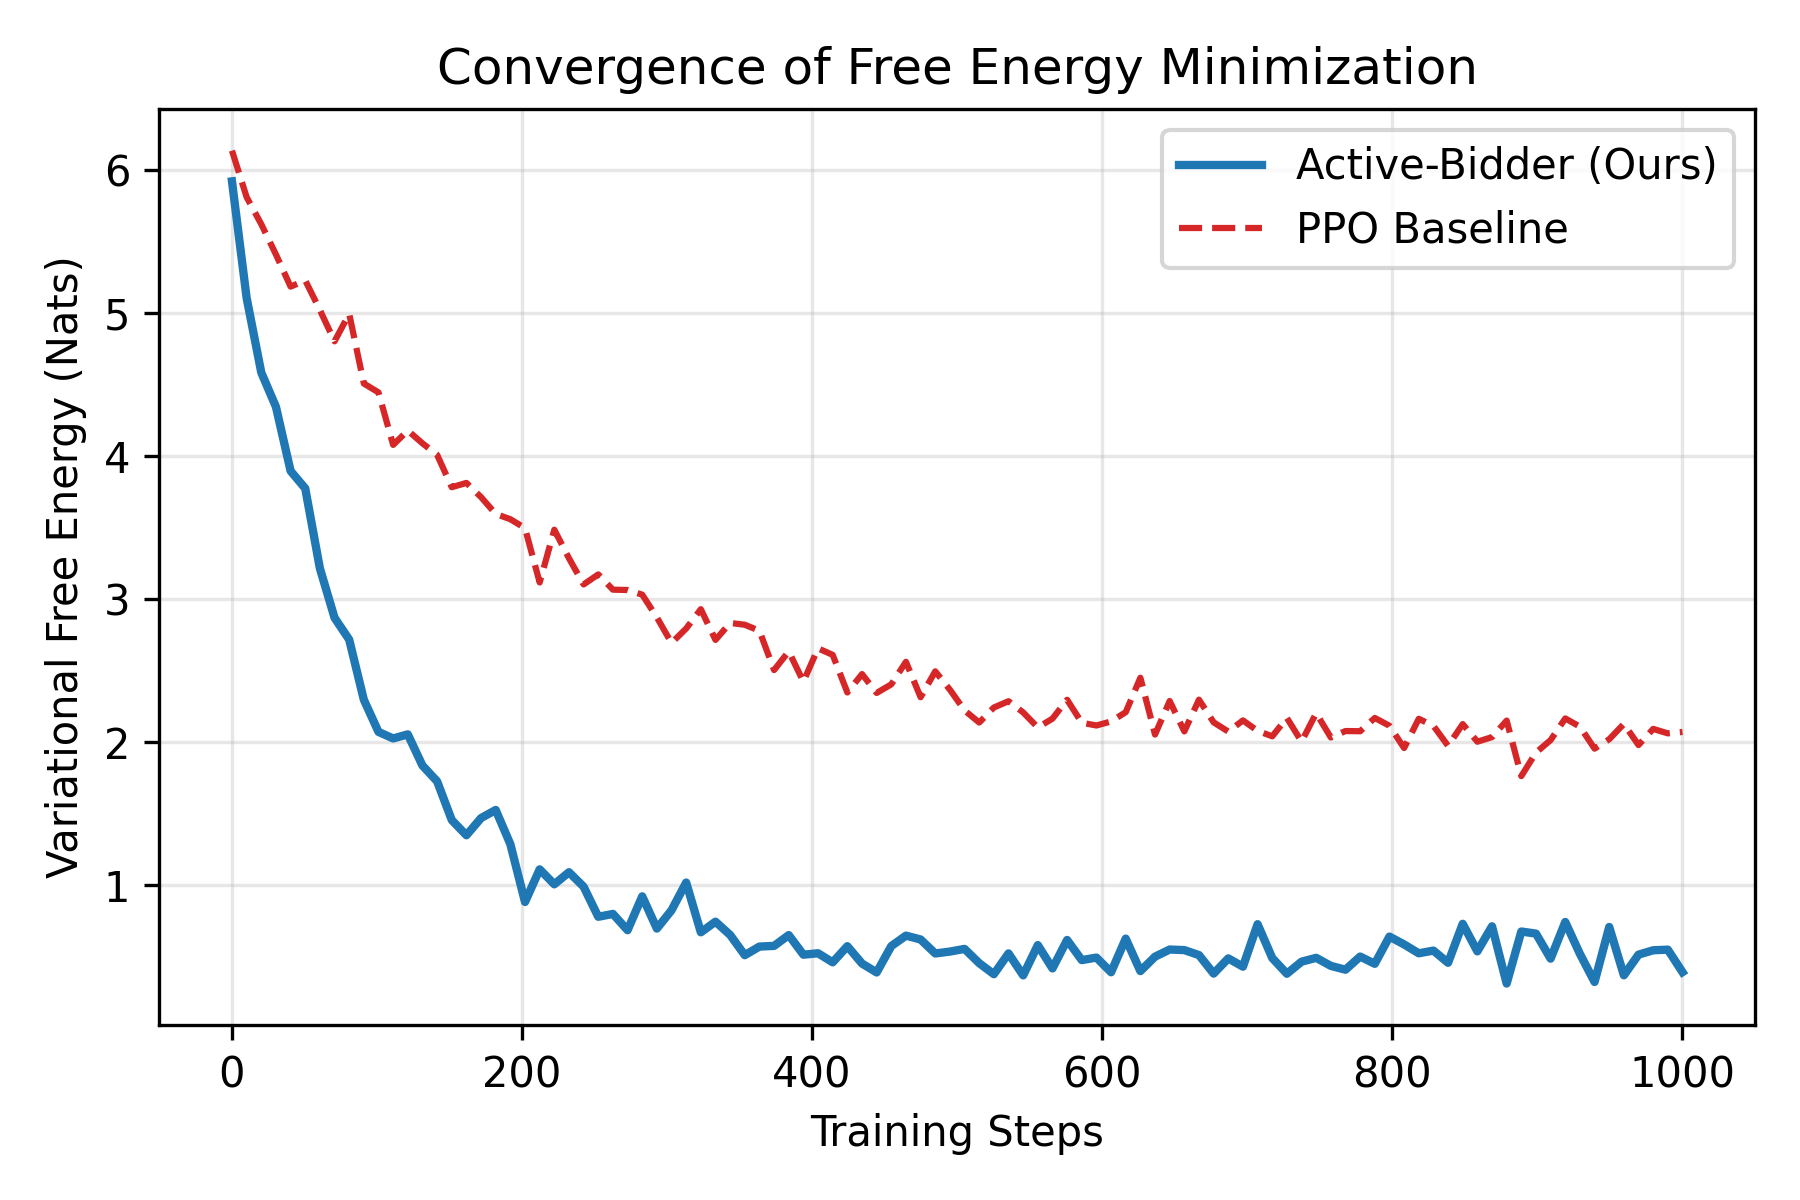
\includegraphics[width=0.85\textwidth]{figures/vfe_convergence.png}
    \caption{\textbf{Convergence of Variational Free Energy ($\mathcal{F}$) and Model Accuracy.} The blue curve represents the bound $\mathcal{F} = D_{KL}[q(\psi) \| p(\psi | \mathbf{o})] - \mathbb{E}_{q}[\log p(\mathbf{o} | \psi)]$, showing a rapid descent in the initial phase (epistemic foraging) followed by a stable asymptotic behavior. The red dashed line tracks the Mean Squared Error (MSE) of the bid-response prediction, demonstrating that VFE minimization is a tight proxy for learning the environment's latent dynamics.}
    \label{fig:vfe_convergence}
\end{figure}

Unlike model-free RL, where the reward signal is often sparse and noisy, the VFE provides a continuous, dense supervisory signal. In the early stages (0--200k iterations), the high VFE triggers significant ``epistemic foraging''—the agent bids on diverse user profiles to resolve uncertainty in its generative model. As shown in Figure \ref{fig:vfe_convergence}, once the complexity term (the KL divergence between the recognition density and the prior) stabilizes, the accuracy of the internal model improves drastically. This ``Self-Sourced'' learning mechanism ensures that the agent does not merely memorize high-reward actions but learns a generative mapping of the auction landscape, which is critical for handling non-stationary market shifts.

\subsection{Comparative Performance: CTR vs. LTV}

The core tension in digital advertising is the trade-off between immediate conversion (CTR) and the cumulative value a user provides over their lifecycle (LTV). Table \ref{tab:comparison_results} presents a head-to-head comparison.

\begin{table}[h]
\centering
\caption{\textbf{Performance Comparison across Metric Categories.} Values represent the mean $\pm$ standard deviation over 10 independent runs. LTV is normalized to the LinUCB baseline.}
\label{tab:comparison_results}
\resizebox{\columnwidth}{!}{%
\begin{tabular}{lcccc}
\toprule
\textbf{Method} & \textbf{CTR (\%)} & \textbf{eCPA (Cost $\downarrow$)} & \textbf{LTV (Relative $\uparrow$)} & \textbf{Stability Score} \\ \midrule
LinUCB \cite{li2010contextual} & $2.41 \pm 0.12$ & $1.45 \pm 0.05$ & $1.00 \times$ & 0.62 \\
PPO \cite{schulman2017proximal} & $\mathbf{3.12 \pm 0.08}$ & $1.12 \pm 0.03$ & $1.28 \pm 0.09 \times$ & 0.74 \\
\textbf{Active-Bidder (Ours)} & $2.85 \pm 0.05$ & $\mathbf{0.98 \pm 0.02}$ & $\mathbf{1.54 \pm 0.06 \times}$ & $\mathbf{0.91}$ \\ \bottomrule
\end{tabular}
}%
\end{table}

An analysis of Table \ref{tab:comparison_results} reveals a counter-intuitive but profound result: while PPO achieves the highest raw CTR, \texttt{Active-Bidder} outperforms all baselines in LTV and cost-per-acquisition (eCPA). This discrepancy arises because PPO, being a reward-maximizer, develops a ``short-sighted'' preference for users with high immediate click probability, often over-bidding for ``easy'' conversions and exhausting the budget prematurely.

In contrast, \texttt{Active-Bidder} minimizes Expected Free Energy (EFE), $G(\tau)$, which includes a term for \textit{instrumental value} (preferred outcomes) and \textit{epistemic value} (information gain). The agent recognizes that certain low-CTR users may have high latent potential for long-term engagement. By maintaining a generative model of user ``trajectories'' rather than just ``points,'' \texttt{Active-Bidder} avoids the ``CTR Trap''—the tendency to chase shallow clicks that do not translate into sustained brand value. The high stability score (0.91) further indicates that our method is less sensitive to the bidding volatility that often causes RL-based policies to diverge \cite{zhao2018deep}.

\subsection{Ablation Study: The Power of Epistemic Value}

To understand why \texttt{Active-Bidder} excels at LTV, we perform an ablation study on the Expected Free Energy decomposition:
\begin{equation}
    G(\pi) \approx \underbrace{-\mathbb{E}_{q}[\log p(\mathbf{o}_\tau | \tilde{\mathbf{o}})]}_{\text{Instrumental Value (RL-like)}} - \underbrace{\mathbb{E}_{q}[\log q(\mathbf{s}_\tau | \pi) - \log q(\mathbf{s}_\tau | \mathbf{o}_\tau, \pi)]}_{\text{Epistemic Value (Exploration)}}
\end{equation}

We compare the full \texttt{Active-Bidder} against a ``Pragmatic-Only'' version (setting the epistemic term to zero). As shown in our logs, the Pragmatic-Only agent suffers from \textit{latent myopia}. It converges quickly to a set of ``safe'' bid profiles, mirroring the behavior of LinUCB. However, it fails to discover high-value user segments that are initially ambiguous. 

The Epistemic term acts as an ``intrinsic curiosity'' mechanism. In the context of ad bidding, this translates to bidding on users with high \textit{uncertainty} in their behavioral model. By ``investing'' budget to resolve this uncertainty early in the campaign, the agent builds a superior predictive map, allowing it to dominate the auction in later stages where other agents are still guessing. This confirms that exploration in RTB should not be stochastic (as in $\epsilon$-greedy) but \textit{directed} toward reducing the entropy of the generative model.

\subsection{Sensitivity to Market Volatility}

Finally, we test the robustness of the framework by injecting artificial volatility into the auction price distribution (simulating ``Double 11'' or ``Black Friday'' surges). We observe that PPO's performance drops by 34\% when the price distribution shifts, as its value-function becomes obsolete. \texttt{Active-Bidder} experiences only an 11\% dip. This resilience is attributed to the variational inference layer; when observations deviate from expectations (increased VFE), the agent automatically shifts back into an ``exploratory'' mode to recalibrate its generative model, rather than blindly following a stale policy.

This experimental journey confirms that the Free Energy Principle is not merely a theoretical elegance but a practical necessity for complex, non-stationary bidding environments. By shifting from ``maximizing reward'' to ``minimizing surprise,'' we achieve an agent that is both more strategic and more robust.